%%% Hlavní soubor. Zde se definují základní parametry a odkazuje se na ostatní části. %%%

%% Verze pro jednostranný tisk:
% Okraje: levý 40mm, pravý 25mm, horní a dolní 25mm
% (ale pozor, LaTeX si sám přidává 1in)
\documentclass[12pt,a4paper]{report}
\setlength\textwidth{145mm}
\setlength\textheight{247mm}
\setlength\oddsidemargin{15mm}
\setlength\evensidemargin{15mm}
\setlength\topmargin{0mm}
\setlength\headsep{0mm}
\setlength\headheight{0mm}
% \openright zařídí, aby následující text začínal na pravé straně knihy
\let\openright=\clearpage

%% Pokud tiskneme oboustranně:
% \documentclass[12pt,a4paper,twoside,openright]{report}
% \setlength\textwidth{145mm}
% \setlength\textheight{247mm}
% \setlength\oddsidemargin{14.2mm}
% \setlength\evensidemargin{0mm}
% \setlength\topmargin{0mm}
% \setlength\headsep{0mm}
% \setlength\headheight{0mm}
% \let\openright=\cleardoublepage
\usepackage[rgb,hyperref,usenames]{xcolor}  % barevná sazba

%% Vytváříme PDF/A-2u
\usepackage[a-2u]{pdfx}

%% Přepneme na českou sazbu a fonty Latin Modern
\usepackage[czech]{babel}
\usepackage{lmodern}
\usepackage[T1]{fontenc}
\usepackage{textcomp}

%% Použité kódování znaků: obvykle latin2, cp1250 nebo utf8:
\usepackage[utf8]{inputenc}

%%% Další užitečné balíčky (jsou součástí běžných distribucí LaTeXu)
\usepackage{amsmath}        % rozšíření pro sazbu matematiky
\usepackage{amsfonts}       % matematické fonty
\usepackage{amsthm}         % sazba vět, definic apod.
\usepackage{bbding}         % balíček s nejrůznějšími symboly
			    % (čtverečky, hvězdičky, tužtičky, nůžtičky, ...)
\usepackage{bm}             % tučné symboly (příkaz \bm)
\usepackage{graphicx}       % vkládání obrázků
\usepackage{fancyvrb}       % vylepšené prostředí pro strojové písmo
\usepackage{indentfirst}    % zavede odsazení 1. odstavce kapitoly
\usepackage{natbib}         % zajištuje možnost odkazovat na literaturu
			    % stylem AUTOR (ROK), resp. AUTOR [ČÍSLO]
\usepackage[nottoc]{tocbibind} % zajistí přidání seznamu literatury,
                            % obrázků a tabulek do obsahu
\usepackage{icomma}         % inteligetní čárka v matematickém módu
\usepackage{dcolumn}        % lepší zarovnání sloupců v tabulkách
\usepackage{booktabs}       % lepší vodorovné linky v tabulkách
\usepackage{paralist}       % lepší enumerate a itemize

%%% Údaje o práci

% Název práce v jazyce práce (přesně podle zadání)
\def\NazevPrace{Extrakce melodice pomocí hlubokého učení}

% Název práce v angličtině
\def\NazevPraceEN{Melody Extraction using Deep Learning}

% Jméno autora
\def\AutorPrace{Jiří Balhar}

% Rok odevzdání
\def\RokOdevzdani{2019}

% Název katedry nebo ústavu, kde byla práce oficiálně zadána
% (dle Organizační struktury MFF UK, případně plný název pracoviště mimo MFF)
\def\Katedra{Ústav formální a aplikované lingvistiky}
\def\KatedraEN{Institute of Formal and Applied Linguistics}

% Jedná se o katedru (department) nebo o ústav (institute)?
\def\TypPracoviste{Ústav}
\def\TypPracovisteEN{Institute}

% Vedoucí práce: Jméno a příjmení s~tituly
\def\Vedouci{Mgr. Jan Hajič}

% Pracoviště vedoucího (opět dle Organizační struktury MFF)
\def\KatedraVedouciho{ústav}
\def\KatedraVedoucihoEN{institute}

% Studijní program a obor
\def\StudijniProgram{Informatika}
\def\StudijniObor{Programování a softwarové systémy}

% Nepovinné poděkování (vedoucímu práce, konzultantovi, tomu, kdo
% zapůjčil software, literaturu apod.)
\def\Podekovani{%
Poděkování.
}

% Abstrakt (doporučený rozsah cca 80-200 slov; nejedná se o zadání práce)
\def\Abstrakt{%
Abstrakt.
}
\def\AbstraktEN{%
Abstract.
}

% 3 až 5 klíčových slov (doporučeno), každé uzavřeno ve složených závorkách
\def\KlicovaSlova{%
{klíčová} {slova}
}
\def\KlicovaSlovaEN{%
{key} {words}
}

%% Balíček hyperref, kterým jdou vyrábět klikací odkazy v PDF,
%% ale hlavně ho používáme k uložení metadat do PDF (včetně obsahu).
%% Většinu nastavítek přednastaví balíček pdfx.
\hypersetup{unicode}
\hypersetup{breaklinks=true}

%% Definice různých užitečných maker (viz popis uvnitř souboru)
%%% Tento soubor obsahuje definice různých užitečných maker a prostředí %%%
%%% Další makra připisujte sem, ať nepřekáží v ostatních souborech.     %%%

%%% Drobné úpravy stylu

% Tato makra přesvědčují mírně ošklivým trikem LaTeX, aby hlavičky kapitol
% sázel příčetněji a nevynechával nad nimi spoustu místa. Směle ignorujte.
\makeatletter
\def\@makechapterhead#1{
  {\parindent \z@ \raggedright \normalfont
   \Huge\bfseries \thechapter. #1
   \par\nobreak
   \vskip 20\p@
}}
\def\@makeschapterhead#1{
  {\parindent \z@ \raggedright \normalfont
   \Huge\bfseries #1
   \par\nobreak
   \vskip 20\p@
}}
\makeatother

% Toto makro definuje kapitolu, která není očíslovaná, ale je uvedena v obsahu.
\def\chapwithtoc#1{
\chapter*{#1}
\addcontentsline{toc}{chapter}{#1}
}

% Trochu volnější nastavení dělení slov, než je default.
\lefthyphenmin=2
\righthyphenmin=2

% Zapne černé "slimáky" na koncích řádků, které přetekly, abychom si
% jich lépe všimli.
\overfullrule=0mm

%%% Makra pro definice, věty, tvrzení, příklady, ... (vyžaduje baliček amsthm)

\theoremstyle{plain}
\newtheorem{veta}{Věta}
\newtheorem{lemma}[veta]{Lemma}
\newtheorem{tvrz}[veta]{Tvrzení}

\theoremstyle{plain}
\newtheorem{definice}{Definice}

\theoremstyle{remark}
\newtheorem*{dusl}{Důsledek}
\newtheorem*{pozn}{Poznámka}
\newtheorem*{prikl}{Příklad}

%%% Prostředí pro důkazy

\newenvironment{dukaz}{
  \par\medskip\noindent
  \textit{Důkaz}.
}{
\newline
\rightline{$\square$}  % nebo \SquareCastShadowBottomRight z balíčku bbding
}

%%% Prostředí pro sazbu kódu, případně vstupu/výstupu počítačových
%%% programů. (Vyžaduje balíček fancyvrb -- fancy verbatim.)

\DefineVerbatimEnvironment{code}{Verbatim}{fontsize=\small, frame=single}

%%% Prostor reálných, resp. přirozených čísel
\newcommand{\R}{\mathbb{R}}
\newcommand{\N}{\mathbb{N}}

%%% Užitečné operátory pro statistiku a pravděpodobnost
\DeclareMathOperator{\pr}{\textsf{P}}
\DeclareMathOperator{\E}{\textsf{E}\,}
\DeclareMathOperator{\var}{\textrm{var}}
\DeclareMathOperator{\sd}{\textrm{sd}}

%%% Příkaz pro transpozici vektoru/matice
\newcommand{\T}[1]{#1^\top}

%%% Vychytávky pro matematiku
\newcommand{\goto}{\rightarrow}
\newcommand{\gotop}{\stackrel{P}{\longrightarrow}}
\newcommand{\maon}[1]{o(n^{#1})}
\newcommand{\abs}[1]{\left|{#1}\right|}
\newcommand{\dint}{\int_0^\tau\!\!\int_0^\tau}
\newcommand{\isqr}[1]{\frac{1}{\sqrt{#1}}}
\newcommand{\argmin}{\operatornamewithlimits{argmin}}
\newcommand{\argmax}{\operatornamewithlimits{argmax}}

%%% Vychytávky pro tabulky
\newcommand{\pulrad}[1]{\raisebox{1.5ex}[0pt]{#1}}
\newcommand{\mc}[1]{\multicolumn{1}{c}{#1}}

%%% Sémantické zkratky
\newcommand{\uloha}[1]{\emph{#1}}
\newcommand{\dataset}[1]{\emph{#1}}

%% Titulní strana a různé povinné informační strany
\begin{document}
%%% Titulní strana práce a další povinné informační strany

%%% Titulní strana práce

\pagestyle{empty}
\hypersetup{pageanchor=false}

\begin{center}

\centerline{\mbox{
\includegraphics[width=166mm]{../img/logo-cs.pdf}}}

\vspace{-8mm}
\vfill

{\bf\Large BAKALÁŘSKÁ PRÁCE}

\vfill

{\LARGE\AutorPrace}

\vspace{15mm}

{\LARGE\bfseries\NazevPrace}

\vfill

\Katedra

\vfill

\begin{tabular}{rl}

Vedoucí bakalářské práce: & \Vedouci \\
\noalign{\vspace{2mm}}
Studijní program: & \StudijniProgram \\
\noalign{\vspace{2mm}}
Studijní obor: & \StudijniObor \\
\end{tabular}

\vfill

% Zde doplňte rok
Praha \RokOdevzdani

\end{center}

\newpage

%%% Následuje vevázaný list -- kopie podepsaného "Zadání bakalářské práce".
%%% Toto zadání NENÍ součástí elektronické verze práce, nescanovat.

%%% Strana s čestným prohlášením k bakalářské práci

\openright
\hypersetup{pageanchor=true}
\pagestyle{plain}
\pagenumbering{roman}
\vglue 0pt plus 1fill

\noindent
Prohlašuji, že jsem tuto bakalářskou práci vypracoval(a) samostatně a výhradně
s~použitím citovaných pramenů, literatury a dalších odborných zdrojů.

\medskip\noindent
Beru na~vědomí, že se na moji práci vztahují práva a povinnosti vyplývající
ze zákona č. 121/2000 Sb., autorského zákona v~platném znění, zejména skutečnost,
že Univerzita Karlova má právo na~uzavření licenční smlouvy o~užití této
práce jako školního díla podle §60 odst. 1 autorského zákona.

\vspace{10mm}

\hbox{\hbox to 0.5\hsize{%
V ........ dne ............
\hss}\hbox to 0.5\hsize{%
Podpis autora
\hss}}

\vspace{20mm}
\newpage

%%% Poděkování

\openright

\noindent
\Podekovani

\newpage

%%% Povinná informační strana bakalářské práce

\openright

\vbox to 0.5\vsize{
\setlength\parindent{0mm}
\setlength\parskip{5mm}

Název práce:
\NazevPrace

Autor:
\AutorPrace

\TypPracoviste:
\Katedra

Vedoucí bakalářské práce:
\Vedouci, \KatedraVedouciho

Abstrakt:
\Abstrakt

Klíčová slova:
\KlicovaSlova

\vss}\nobreak\vbox to 0.49\vsize{
\setlength\parindent{0mm}
\setlength\parskip{5mm}

Title:
\NazevPraceEN

Author:
\AutorPrace

\TypPracovisteEN:
\KatedraEN

Supervisor:
\Vedouci, \KatedraVedoucihoEN

Abstract:
\AbstraktEN

Keywords:
\KlicovaSlovaEN

\vss}

\newpage

\openright
\pagestyle{plain}
\pagenumbering{arabic}
\setcounter{page}{1}


%%% Strana s automaticky generovaným obsahem bakalářské práce

\tableofcontents

%%% Jednotlivé kapitoly práce jsou pro přehlednost uloženy v samostatných souborech
\chapter{Úvod}\label{chap:uvod}
\addcontentsline{toc}{chapter}{Úvod}

Spolu s harmonií a rytmem představuje melodie základní stavební kámen většiny existující hudby. V průběhu vývoje od folklórních zpěvů přes orchestrální skladby po soudobou elektroniku si melodie téměř vždy zachovávala své dominantní postavení nositele esence jednotlivých písní. Melodie je to hlavní, co si člověk po poslechu skladby odnáší a nejsnadněji vybaví, a její důležitost je zejména v našem kulturním kontextu natolik jednoznačná, že se hudba, která ji postrádá, zřídkakdy dostává do širokého povědomí.

\begin{figure}[h]\centering
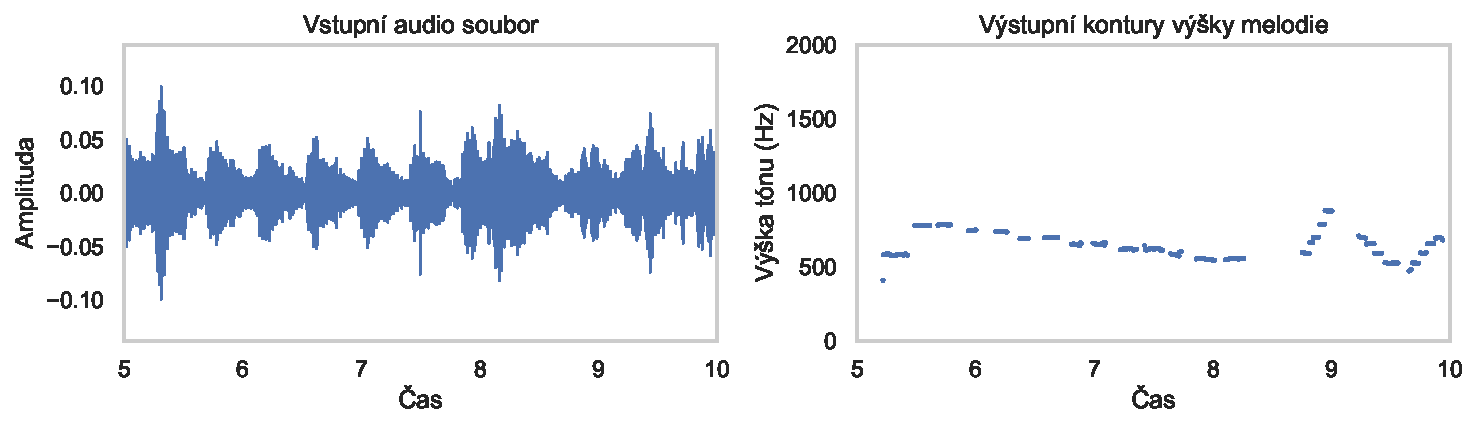
\includegraphics[width=\textwidth,height=\textheight,keepaspectratio]{../img/input_output}
\caption{Příklad vstupu a výstupu metody pro extrakci melodie. \textcolor{red}{přidat zvukový přílkad do přílohy}}
\label{obr:input_output}
\end{figure}

Tato práce se zabývá metodami odhadu fundamentální frekvence melodie ze zvukové nahrávky. Jinými slovy je naším cílem získat v každém bodě vstupní skladby informaci o tom, zda melodie v daném okamžiku zní a její případnou výšku. Jde o jednu z nejdůležitějších a zároveň nejtěžších úloh z oboru \textit{Music Information Retrieval} (MIR), jejíž rozsah využití v této doméně pokrývá významnou část aktivně řešených, otevřených problémů. 

Spolehlivý přepis melodie by usnadnil vyhledávání v hudebních datech, ať už na základě notového zápisu (\textit{Symbolic Melodic Similarity}), pomocí nekvalitní nahrávky z rádia (\textit{Audio Fingerprinting}), pomocí broukání (\textit{Query by Singing/Humming}) nebo dokonce pomocí coveru hledané písně (\textit{Audio Cover Song Identification}). Mimo vyhledávání by byl algoritmus užitečný pro další zpracování zvukového signálu, ať už pro manipulaci a úpravu melodického hlasu (například software Melodyne), nebo naopak jeho odstranění a vytvoření karaoke doprovodu (\textit{Informed Source Separation}). V neposlední řadě by extrakce melodie pomohla při kategorizaci hudebních dat, například podle žánru (\textit{Genre Classification}) nebo podle zpěváka (\textit{Singer Characterization}). A konečně široké spektrum využití by nalezla i v muzikologii (případně etnomuzikologii) pro kvantitativní i kvalitativní studii hudebních motivů a postupů (V jazzu například \cite{Pfleiderer}).

Extrakce melodie však nemusí sloužit pouze jako mezikrok pro řešení jiné úlohy, užitečný je i samotný výstup algoritmu, znázorněný na obrázku \ref{obr:input_output}. Motivačním příkladem použití může být pomoc při transkripci. Představíme-li si začínajícího hráče na saxofon, který si chce do not přepsat své oblíbené jazzové sólo, výstup algoritmu mu dá užitečnou informaci o tom, jaký tón zní v jakou chvíli. Z této reprezentace už pak hráči zbývá nalezené tóny projít a zapsat je do notové osnovy.

\section{Analýza hudebního signálu}

Proč je ale extrakce melodie otevřený problém? Příbuzná úloha, která spočívá v přepisu nahrávky jednoho izolovaného nástroje, je v podstatě vyřešena \citep{Mauch2014a}, proč se tato úloha po přidání hudebního doprovodu stává výrazně obtížnější? Pro vysvětlení zásadního problému, který se s přepisem nahrávky pojí, musíme nejdříve přiblížit vůbec povahu zvuku a možnosti jeho zkoumání.

Naše zkušenost se zvukem probíhá primárně skrze sluch. Teprve na hlasitém koncertu však člověk pocítí, že zvuk je ve své fyzikální podstatě změna tlaku vzduchu, putující od zdroje k posluchači. Díky sluchu z těchto vibrací dokážeme oddělit jednotlivé zdroje a identifikovat v nich i velmi jemné rozdíly. Ačkoli jde o subjektivní vjemy, zvuky lze částečně rozřadit podle toho, jak snadno v nich rozeznáme nějakou konkrétní výšku. 

\vspace*{0.5cm}

Čtenář této práce si nyní může postupně vybavit: hrající violoncello, odbíjení kostelního zvonu, cinknutí příboru, štěkot psa, plynutí potoka, šelest listí stromů, trhání papíru, tlesknutí a prasknutí balónku.

\vspace*{0.5cm}

Se ztrácející se zřetelností výšky nejprve přijdeme o možnost zpívat společně se zdrojem zvuku v harmonii a posléze i o možnost si představit \uv{vyšší} a \uv{nižší} instance toho samého zvuku (jak zní vysoké a nízké prasknutí balónku?). To, co mají první z uvedených příkladů společné, je výrazná a stabilní periodicita jejich signálu --- daný tlakový průběh se opakuje v čase. Díky sluchu tuto periodicitu interpretujeme jako výšku, přičemž různé výšky se od sebe liší frekvencí, se kterou se signál opakuje. Hudební nástroje jsou jedním ze zdrojů těchto pravidelných vibrací, jejichž frekvenci lze zpravidla měnit (pomocí klapek, pohybu prstu po struně, atd.). Hlas nástroje však není charakteristický pouze svou výškou, nýbrž i barvou. Ta je určena podobou signálu v rámci jedné periody. 

\begin{figure}[h]\centering
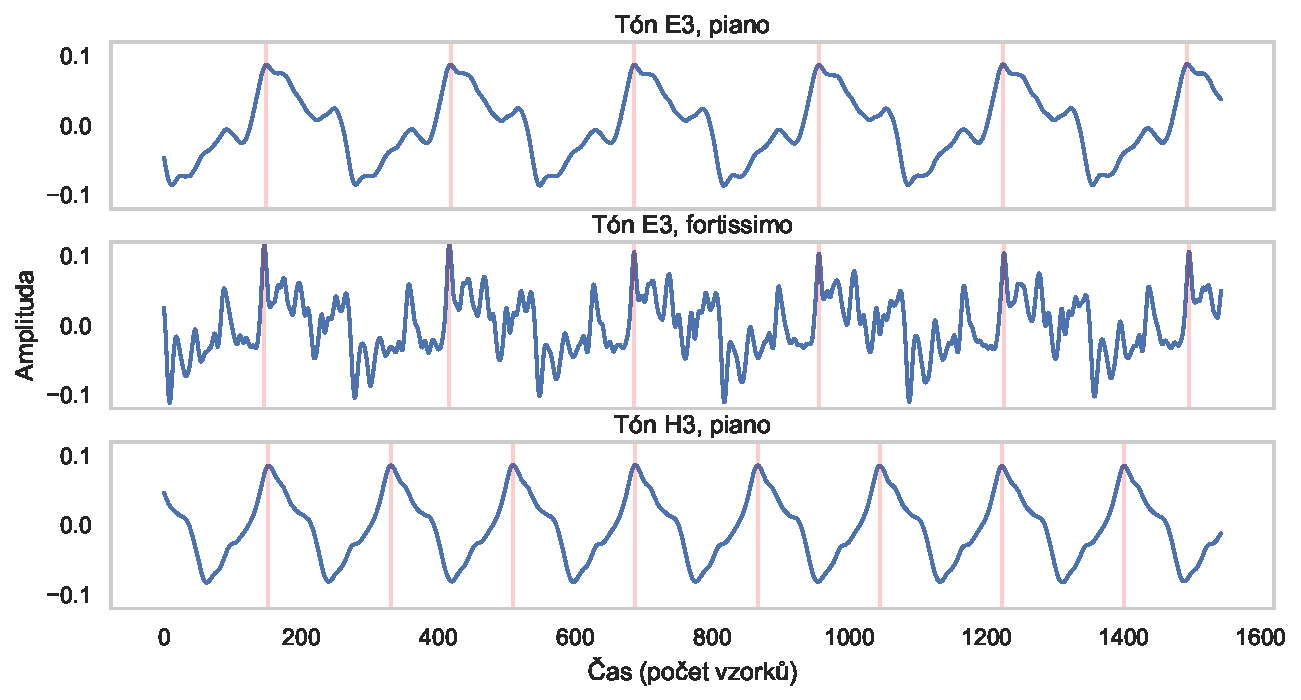
\includegraphics[width=\textwidth,height=\textheight,keepaspectratio]{../img/audio_clarinet}
\caption{Zvuk klarinetu, tóny s různou výškou a dynamikou, 35 milisekund signálu se vzorkovací frekvencí $44\,100\,\rm Hz$. \textcolor{red}{nějak uvést zdroj zvuku \url{https://www.philharmonia.co.uk/explore/sound_samples/clarinet?p=3}}}
\label{obr:audio_clarinet}
\end{figure}

Na obrázku \ref{obr:audio_clarinet} můžeme srovnat tři tóny hrané klarinetem, první dva mají stejnou výšku, jsou ale zahrané s různou intenzitou (dynamikou) \textcolor{red}{je tohle správně formulované, vím že dynamika není intenzita, ale \uv{zahrané s různou dynamikou} mi zní divně?}. Jejich vizuální rozdíl částečně odpovídá i rozdílu v barvě tónu, první tón má příjemný, měkký zvuk; druhý je výraznější a hrubší. Třetí tón se od zbylých liší svou výškou, což lze pozorovat na kratší periodě signálu, která je na obrázku vyznačená úsečkami. 

\begin{figure}[h]\centering
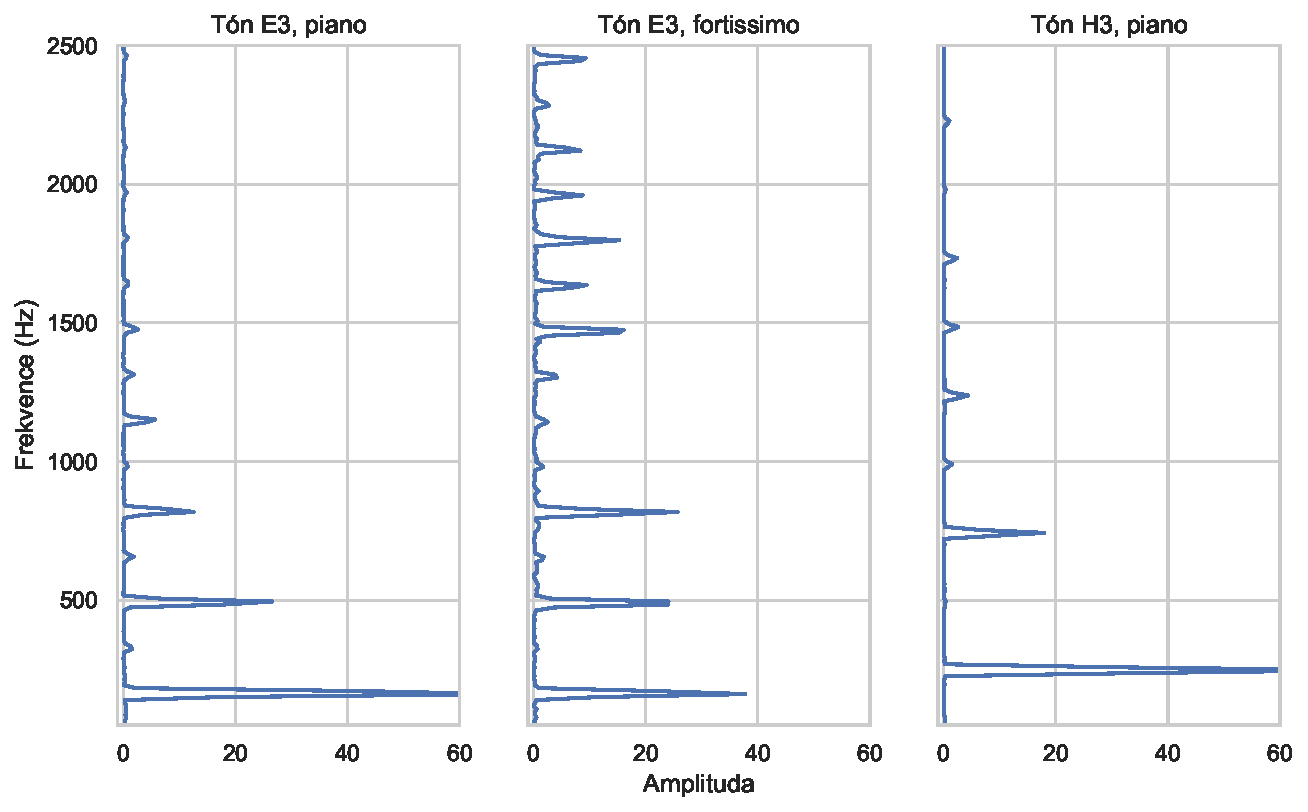
\includegraphics[width=\textwidth,height=\textheight,keepaspectratio]{../img/audio_clarinet_dft}
\caption{Zvuk klarinetu, absolutní hodnota výstupu Fourierovy tranformace signálu délky 4096 s oknem typu Hamming.}
\label{obr:audio_clarinet_dft}
\end{figure}

Jedním ze způsobů analýzy zvukového signálu je pomocí Fourierovy transformace (DFT). Základní myšlenkou je, že na signál lze hledět jako na vážený součet jednodušších signálů. Podobně, jako když se barvy na obrazovce míchají ze tří základních, libovolný zvuk můžeme smíchat ze sady sinusoid. Výslednou kombinaci všech frekvencí, ze kterých se zvuk skládá, označujeme \emph{zvukové spektrum}. Na obrázku \ref{obr:audio_clarinet_dft} vidíme část výsledku Fourierovy transformace zvuků klarinetu z předchozího příkladu. To zásadní, co na spektru tónu můžeme pozorovat, je jeho podstata jakožto součet \emph{harmonických složek}. Tón, kterému posluchač přisoudí výšku $f_0$, se zpravidla skládá ze součtu sinusoid, jejichž frekvence je celočíselným násobkem základní frekvence $f_0$ (jinak také nazývaná \emph{fundamentální frekvence}). Například tedy tón E3 se na obrázku \ref{obr:audio_clarinet_dft} skládá ze složek o frekvenci $165\,\rm Hz$, $330\,\rm Hz$, $495\,\rm Hz$, \dots, zároveň intenzita těchto harmonických frekvencí určuje barvu hlasu.

Ukazuje se, že práce s touto reprezentací zvuku je pro analýzu signálu užitečnější, než práce s nezpracovaným signálem. Ze spektrální reprezentace je například na první pohled zřejmý vztah fundamentálních frekvencí porovnávaných signálů, který odpovídá lidské intuici o výšce zvuků --- tón H3 je na obrázku \ref{obr:audio_clarinet_dft} opravdu \uv{výše} než tón E3. Díky spektrální analýze lze také pozorovat charakteristiky hlasů různých nástrojů. Pro hlas klarinetu platí, že liché harmonické frekvence jsou mnohem výraznější než sudé (na obrázku \ref{obr:audio_clarinet_dft} vypadají sudé harmonické jako malé vrcholky mezi výraznými lichými), naopak například lidský zpěv je charakteristický výraznějšími sudými harmonickými složkami. Další výhodou je možnost hledání rozdílů v barvě tónů --- na spektru vidíme, že vyšší harmonické jsou u tónu hraném fortissimo mnohem výraznější než u tónu hraném piano. Tyto vyšší frekvence způsobují zmiňovanou hrubost tónu. \textcolor{red}{a tohle se dá říct? Tón hraný fortissimo/piano. Moje znalosti hudební terminologie jsou nulové}

Harmonická struktura, která je vlastní lidskému hlasu a téměř všem zvukům hudebních nástrojů, je zásadní pro metody extrakce melodie. Je to vlastnost, která zvuky potenciálně nesoucí melodii odlišuje od bubnového doprovodu, od šumu nebo od jiných nemelodických rušení. Díky ní se také můžeme pokoušet rozložit souzvuk různě vysokých tónů na jejich původní, čisté signály. 

\textcolor{red}{spektrogram hudby - basa, zpěv a bubny. Pod tím obrázek kompletního přepisu melodických kontur}

\begin{figure}[h]\centering
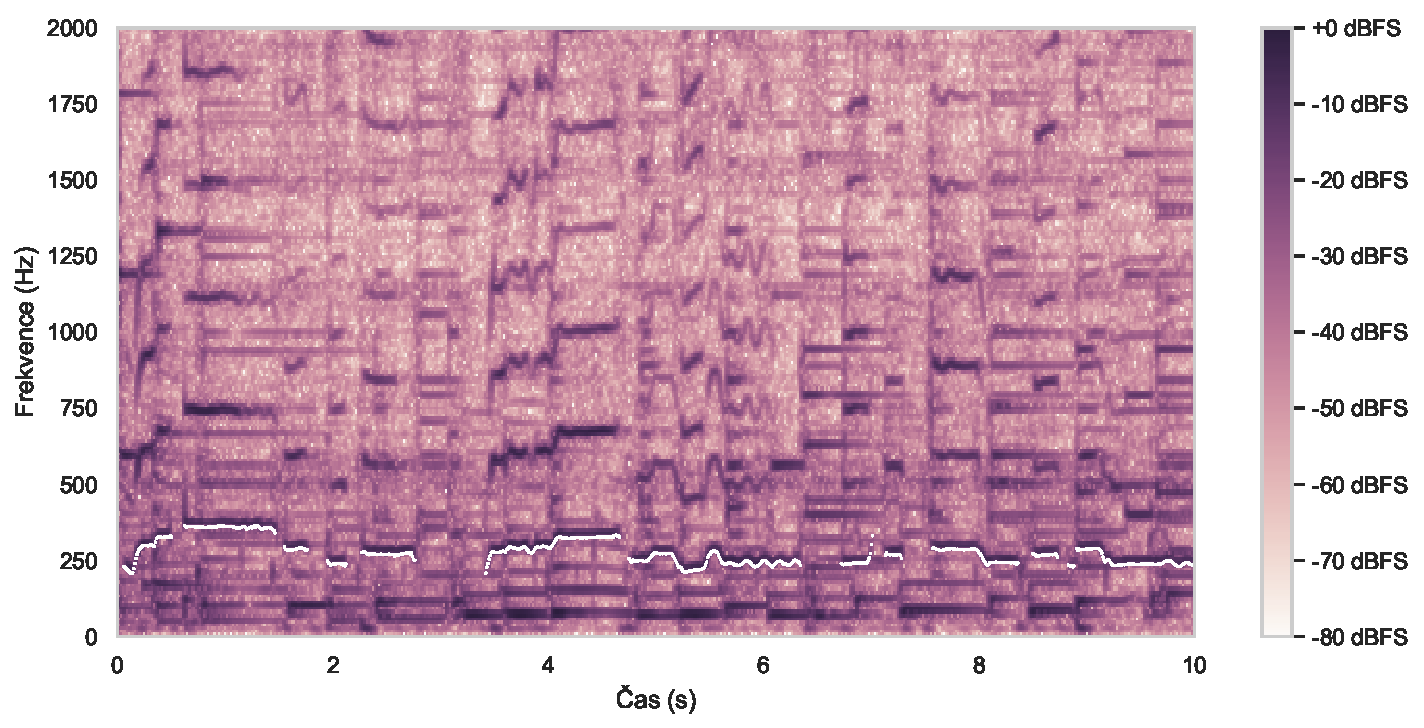
\includegraphics[width=\textwidth,height=\textheight,keepaspectratio]{../img/audio_mix_stft}
\caption{Spektrogram zpěvu s doprovodem piana, basy a perkusí; zpívaná melodie je vyznačena bílým obrysem.}
\label{obr:audio_mix_stft}
\end{figure}

Obrázek \ref{obr:audio_mix_stft} vznikl pomocí opakované Fourierovy transformace, která byla aplikována na po sobě jdoucí, krátké časové úseky vstupní nahrávky, přičemž intenzity frekvenčních složek v každém časovém okamžiku zvuku jsou nyní znázorněny odstínem barvy. Časově-frekvenční reprezentaci signálu nazýváme obecně \emph{spektrogram}, a jeho výpočet je prvním krokem většiny metod pro extrakci melodie.

Na spektrogramu \ref{obr:audio_mix_stft} můžeme pozorovat harmonické struktury tónů --- vyznačenou konturu hlasu, která se na frekvenční ose pohybuje volněji, a pak klavírní a basový doprovod, charakteristický frekvenční stabilitou a v čase slábnoucí amplitudou. Na tomto jednoduchém příkladu lze melodii zpozorovat poměrně snadno, nese ji velmi výrazný, v poměru k doprovodu nejsilnější hlas. Lze na něm však prezentovat první ze základních problémů extrakce melodie.

Frekvence tónů, ze kterých se skládá hudební skladba, jsou uspořádány do stupnic, které definují pevně dané poměry (hudební \emph{intervaly}), ve kterých se tyto tóny ve skladbě mohou vyskytovat. Principem libozvučnosti jsou však takové intervaly, které způsobují, že harmonické frekvence jednotlivých tónů se překrývají a ve výsledné směsi pak není zřejmé, zda-li daná harmonická frekvence patří k jednomu, či více hlasů. Hudební doprovod, pro lidské ucho znějící \uv{pod melodií}, tedy často svými harmonickými frekvencemi zasahuje do melodie samotné, což je zřejmé ze spektrální analýzy.

Dekompozice signálu na jednotlivé znějící hlasy, která je pro člověka přirozená podobně, jako porozumění řeči v rušné kavárně, se kvůli této harmonické povaze tónů a intervalů stává pro algoritmy extrakce melodie obtížným problémem. To, co pro nás činí hudbu zajímavou pro poslech, ji činí obtížně analyzovatelnou pro počítač.


% * další nepříjemnosti
%     * rezonance nástroje po zahrání tónu
%     * dozvuk místnosti
%     * rušení z perkusí
%     * mastering = sice je nahrávka více vyrovnaná, ale problémy přepisu ještě zesiluje
%         * digitální reverb (= dále rozostřuje hranice mezi začátky a konci not, zvětšuje míru překryvů zahraných not)
%         * dynamic range compression = komprese dynamiky zvukového signálu = zmenšuje rozdíly mezi tichými a hlasitými zdroji zvuku
%             * Komprese dynamiky zvukového signálu je proces používaný v audiotechnice ke zmenšení dynamického rozsahu zpracovávaného signálu

\begin{figure}[h]\centering
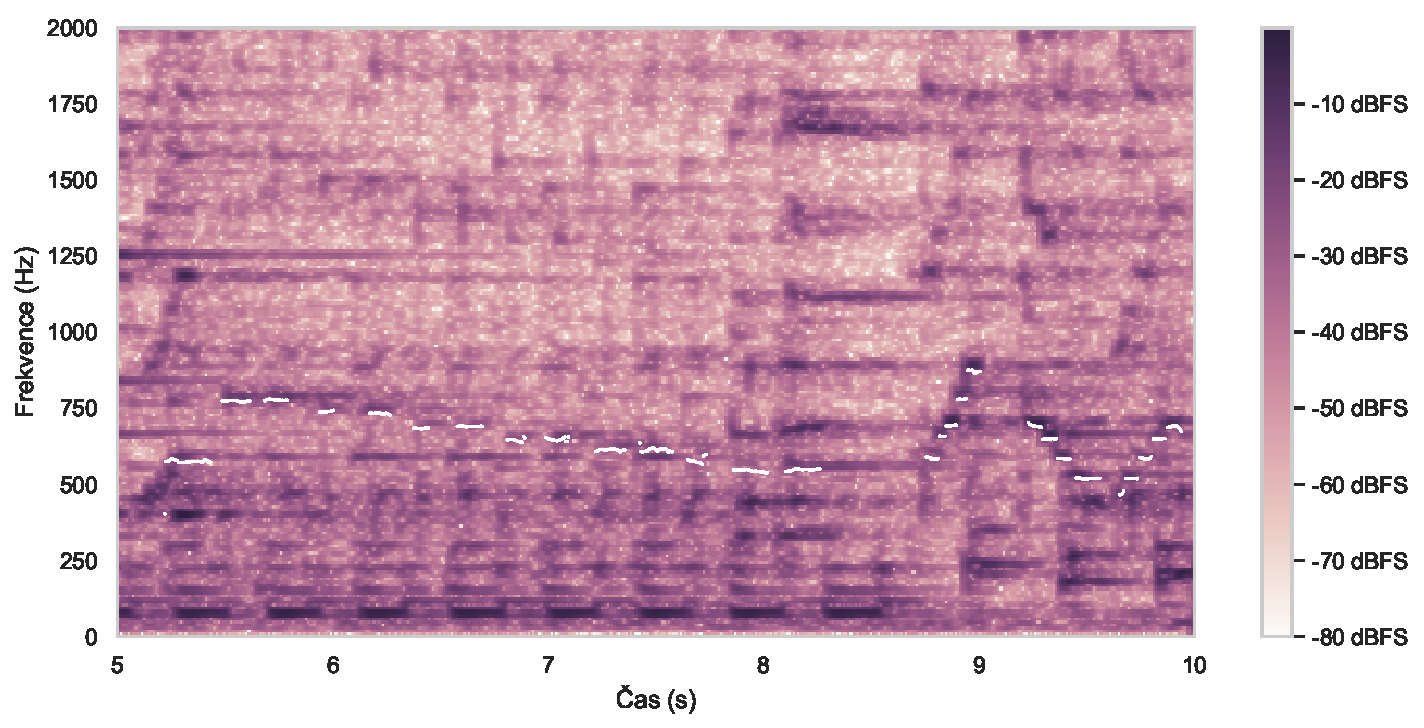
\includegraphics[width=\textwidth,height=\textheight,keepaspectratio]{../img/audio_mix_stft_2}
\caption{Spektrogram orchestrální skladby s obtížně detekovatelnou melodií.}
\label{obr:audio_mix_stft_2}
\end{figure}

\section{Definice melodie}

Rozpoznání melodie v rámci hudební skladby je pro většinu posluchačů intuitivní schopností, která je součástí prožitku poslechu hudby, a která jejímu poslechu vůbec dává smysl. Ačkoli je melodie tedy termín, který je subjektivně jasný, formální, obecně přijímanou muzikologickou definici, která by se zpětně neodkazovala k posluchači, nemá. 

Z tohoto důvodu si výzkumné týmy zabývající se automatickou transkripcí melodie volí pragmaticky spíše užší definice melodie, se kterými se v jejich kontextu pracuje lépe. Práce \cite{Goto1999}, která je považována za jednu z prvních prací v oboru, chápe melodii jako \uv{konturu fundamentální frekvence sestávající se z nejsilnějších tónů hrajících v omezeném frekvenčním rozsahu}. Práce se tedy omezuje na poměrně úzké chápání melodie, obecně se totiž tóny melodie jistě mohou vyskytovat i mimo autory specifikovaný frekvenční rozsah a také nemusí být vždy v poměru s doprovodem nejhlasitější složkou signálu. Z technického hlediska však umožnila autorům implementaci algoritmu běžícího v reálném čase, který poskytoval sémanticky bohatý popis vstupních nahrávek. Navazující články již pracují s volnějšími definicemi, které lépe reflektují podstatu melodie. 

Kompromisem mezi subjektivní a praktickou definicí se na dlouhou dobu stala \uv{extrakce základní frekvence hlavního, neměnného, melodického hlasu}. Ačkoli melodii v reálném hudebním materiálu obvykle nese více hlasů, které se v hraní střídají (například píseň se zpěvem a kytarovým sólem), v letech 2005 -- 2015 se v soutěži MIREX (mezinárodní soutěž pro metody řešící MIR úlohy) provádí evaluace pouze nad krátkými výňatky, kde tato definice není omezující. Přestože se může na první pohled zdát, že tato definice pouze uměle zjednodušuje celou úlohu, její formulace vede k rozvoji nových a zajímavých přístupů, které se sice formálně soustředí právě na extrakci pouze jednoho neměnného hlasu, ale ve výsledku překvapivě dobře fungují i na složitější skladby. Příkladem nového směru může být extrakce melodie pomocí modelování hudebního záznamu jako součtu signálu jednoho hlasu a doprovodu (práce \cite{Durrieu2010} nebo \cite{Bosch2016b}) s přesahem do příbuzné úlohy oddělení hlasů (source separation). Některé práce se zaměřují ještě konkrétněji na separaci lidského zpěvu a doprovodu (\cite{Hsu2010}, \cite{Ikemiya2016}). Nově se také objevují práce, které \uv{hlavní} melodický hlas neinterpretují nutně jako \uv{nejsilnější} a k jeho rozlišení využívají dalších rysů, jako je barva, vibrato nebo délka not. Například \cite{Salamon2012a} využívají těchto rysů pro finální výběr mezi extrahovanými kandidátními konturami.

Ve svém přehledovém článku \cite{Salamon2014} dochází k závěru že výzkum začal v letech 2009--2012 stagnovat, nová data jsou proto pro další vývoj oboru zásadní. Výrazným posunem v rámci MIR komunity proto bylo zveřejnění nových datasetů MedleyDB \citep{Bittner2014} a ORCHSET \citep{Bosch2016}, oba obsahují data, ve kterých již melodii nenese pouze jeden hlas po celou dobu skladby. V porovnání s do té doby dostupnými daty jde také o mnohem rozmanitější kolekce a v případě MedleyDB jde o první volně dostupný dataset, ve kterém se objevují celé skladby, nikoli pouze výňatky.

\cite{Bosch2016} pro práci na datasetu ORCHSET definuje melodii jako \uv{jednohlasou sekvenci tónů, kterou bude posluchač nejspíše reprodukovat, pokud jej požádáme o zapískání či zabroukání příslušné skladby} (na základě článku \cite{Poliner2007}), pro sestavení kolekce dat proto opravdu využívá skupiny posluchačů, které po poslechu krátkých ukázek orchestrální hudby následně žádá o přezpívání melodie. V případě MedleyDB se na anotacích melodie podílí skupina profesionálních hudebníků a vznikají tři různé přepisy melodie s různě volnými formulacemi definice melodie.

Celkový směr výzkumu je tak ve výsledku velmi podmíněn dostupnými daty. Ta tvoří jakýsi protipól k ryze technickým a objektivním cílům algoritmických metod. Nadějí je, že tato dialektika vývoje algoritmů a práce na datech vyústí jednak v metody extrakce, které věrně zachycují podstatu subjektivního prožitku porozumění hudbě, a jednak v celkovém důsledku také snad v lepší porozumění pojmu melodie obecně.

\section{Metody extrakce melodie}

\begin{figure}[h]\centering
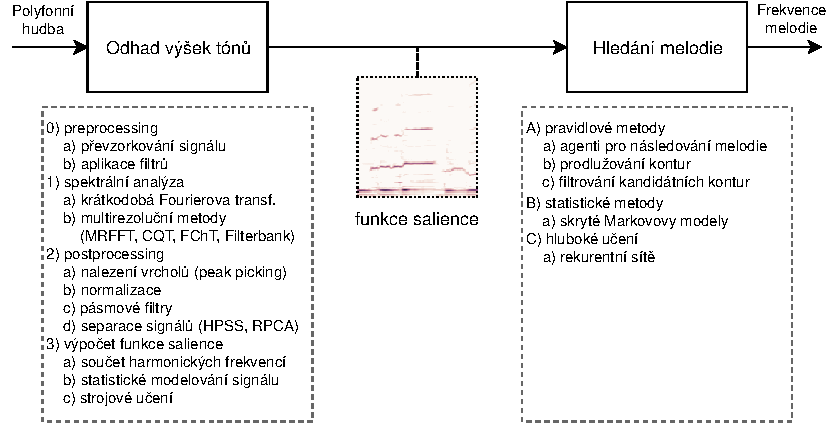
\includegraphics[width=\textwidth,height=\textheight,keepaspectratio]{../img/diagram_systemy_ME}
\caption{Diagram obvyklého návrhu metod pro extrakci melodie.}
\label{obr:diagram_systemy_ME}
\end{figure}

Základním a společným přístupem k problému extrakce melodie je dekompozice na podproblémy odhadu výšek všech znějících hlasů v signálu a následného výběru melodické linie z těchto kandidátních kontur. Jednotlivé metody se pak liší ve způsobech řešení těchto podproblémů, mimo jiné také v míře abstrakce od původního signálu, které při zpracovávání dosahují --- zatímco některé přístupy po celou dobu pracují pouze se signálem jako takovým a důmyslnými způsoby ho transformují tak, aby získaly co nejpřesnější odhad výšky melodie, jiné metody při výpočtu vytváří symbolický popis jednotlivých not a následně i celých frází a melodii pak hledají v tomto vysokoúrovňovém popisu nahrávky. Shrnutí používaných přístupů, blíže popsaných v kapitole \hyperref[chap:souvisejici]{Související práce}, můžeme vidět na diagramu \ref{obr:diagram_systemy_ME}.

\begin{figure}[h]\centering
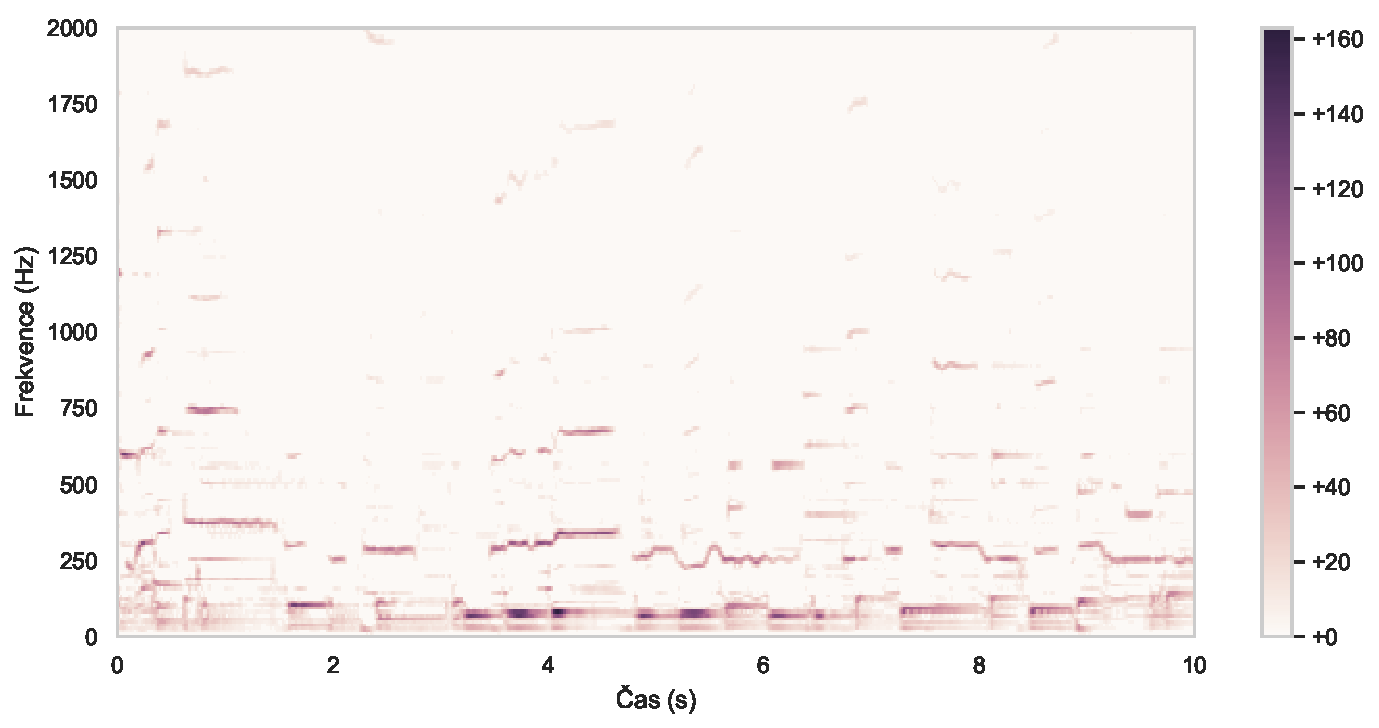
\includegraphics[width=\textwidth,height=\textheight,keepaspectratio]{../img/salience}
\caption{Příklad výstupu výpočtu salienční funkce pomocí váženého sčítání harmonických frekvencí. Ačkoli je zpěv velmi zvýrazněn a salienční funkce na většině nahrávky dobře zachycuje výšku znějící melodie, doprovod kolem čtvrté sekundy nahrávky má vyšší hodnotu než zpěv, což neodpovídá lidskému vnímání zpěvu jakožto nejdůležitější složky signálu.}
\label{obr:salience}
\end{figure}

Prvním krokem všech existujících metod pro extrakci melodie je převod zvukového signálu do frekvenční domény, ať už pomocí zmiňované STFT nebo použitím jiných metod vyvinutých pro analýzu harmonického signálu (MRFFT, CQT, FChT, \dots). Jednou z hlavních výhod těchto dalších metod je logaritmická osa frekvence, díky které je snadné pracovat s harmonickými poměry a hudebními intervaly nezávislé na výšce frekvence. Abychom tuto vlastnost ilustrovali, uvedeme příklad --- tóny A4 a E5 jsou vzdálené o kvintu (na klavíru od tónu A4 musíme postupně zmáčknout 7 bílých a černých klapek, abychom se dostali k tónu E5), tóny A5 a E6 jsou také vzdálené o kvintu. Rozdíl frekvencí těchto tónů je však $220\,\rm Hz$ mezi první dvojicí a $440\,\rm Hz$ mezi druhou dvojicí, tudíž vzdálenost frekvencí daného intervalu závisí na tónu, od kterého se tento interval počítá. Protože je hudební interval jistý \emph{poměr} mezi dvěma tóny, použitím logaritmické osy frekvence se tyto poměry budou jevit jako absolutní rozdíly ($\log n f_0 = \log n + \log f_0$). 

Zpracováním spektrogramu vstupu pak vzniká tzv. \emph{funkce salience}, která každé znějící frekvenci v signálu přiřazuje jisté ohodnocení, které vyjadřuje poměrnou důležitost dané frekvence k ostatním slyšitelným složkám. Funkce salience je tedy v jistém slova smyslu speciální frekvenčně-časová transformace, která podává zejména informace o znějící melodii, nikoli o celkové kompozici signálu. Na obrázku \ref{obr:salience} můžeme srovnat funkci salience vypočtenou pomocí váženého součtu harmonických frekvencí se vstupním spektrogramem \ref{obr:audio_mix_stft}.

Druhým krokem je pak výběr melodie na základě funkce salience. Triviálním řešením je výběr takových frekvencí, které mají nejvyšší ohodnocení. Problémem tohoto přístupu je však to, že jakmile signál obsahuje více podobně ohodnocených tónů, výstup tohoto řešení má tendenci mezi těmito kandidáty často \uv{přeskakovat}. Algoritmy pro extrakci melodie proto volí různě pokročilé metody vyhlazování, případně metody hledání nejpravděpodobnějšího průchodu posloupností stavů (například pomocí Viterbiho algoritmu).

\section{Hluboké učení}

Motivací pro použití metod strojového učení je překonání limitů člověkem navržených, rigidních, pravidlových systémů. Cílem je automatické nalezení optimálního postupu pro řešení úlohy, na základě množství dat, ve kterých strojové učení dokáže nalézt a využít jejich pravidelností. V našem případě pak po metodě založené na strojovém učení požadujeme, aby na základě příkladů z trénovací množiny vytvořila funkci salience.

Výhodou tohoto přístupu je, že o vstupních datech nemusíme dělat žádné předpoklady. Vzniklá metoda pak může v praxi zohledňovat více faktorů ovlivňujících přítomnost melodie, jako je její barva, frekvenční modulace (vibrato, glissando) nebo hlubší vzájemné srovnání současně znějících tónů. Na základě trénovacích příkladů může být tato metoda robustnější vůči většímu spektru barev hlasů nástrojů --- zatímco předešlé metody pro extrakci melodie často uvažují signály s postupně se snižujícím podílem harmonických frekvencí, opravdové signály hudebních nástrojů často tento předpoklad nesplňují (viz obrázek \ref{obr:audio_clarinet_dft}).

První pokus o využití těchto metod představili \cite{Poliner}, vstupní signál transformovali pomocí krátkodobé Fourierovy transformace a část spektra po jednoduché normalizaci použili jako vstupní data pro metodu podpůrných vektorů (SVM). Jejich metoda měla své limitace, výstup byl kvantizován na úroveň jednoho půltónu a tudíž metoda nedokázala dobře postihnout například vibrata. I přesto však tým dosáhl srovnatelných výsledků s ostatními metodami. 

Po roce 2005 jakékoli pokusy o aplikaci strojového učení ustávají a na nové metody se čeká až do roku 2016, jedním z důvodů byl jistě nedostatek dat, tuto situaci zlepšil například dataset MedleyDB \citep{Bittner2014} nebo dnes již zaniklý iKala \citep{Chan2015}. Zájem o strojové učení však znovu stoupá, také díky úspěšnému využití hlubokých neuronových sítí napříč ostatními obory. Na konferenci ISMIR 2016\footnote{International Society for Music Information Retrieval Conference} objevují dva články týmů \cite{Kum2016} a \cite{Rigaud2016}, založené právě na hlubokém učení. V roce 2017 publikuje své metody \cite{Bittner2017} (ISMIR), \cite{Balke2017} (ICASSP\footnote{International Conference on Acoustics, Speech, and Signal Processing}), následující rok přináší metody \cite{DBasaranSEssid2018} (ISMIR), \cite{Bittner2018}. Všechny zmíněné popisujeme v kapitole \hyperref[chap:souvisejici]{Související práce}. V oboru lze tedy od roku 2016 vidět velmi výrazný trend právě směrem k hlubokému učení, a stejný směr je patrný i v příbuzných úlohách přepisu hudby. Tým z laboratoře Google Brain dokázal výrazně zlepšit přepis klavírních skladeb pomocí kombinace konvoluční a rekurentní architektury \citep{Hawthorne2018}. Neuronové sítě také zlepšují výsledky na poli oddělení signálů \citep{Stoller2018}.

V této práci se pokusíme navázat na zmiňované práce a otestovat nové architektury hlubokých neuronových sítí pro úlohu extrakce melodie, zejména pak pro hledání nových způsobů výpočtu funkce salience, v menší míře také pro detekci melodie.

\section{Přínosy práce}

\textcolor{red}{TODO}

\section{Struktura práce}

\textcolor{red}{napsat signpost}

% \cite{Thickstun2016} - musicnet
% \cite{Hawthorne2018} - google magenta

% V oboru transkripce hudby se trend v použití hlubokých sítí
\chapter{Datasety}

Nedostupnost dostatečného množství dat pro automatickou transkripci melodie představuje zejména pro metody strojového učení otevřený problém. Zatímco pro vzdáleně příbuznou úlohu automatického přepisu mluveného slova existuje tisíce hodin nahrávek (například dataset LibriSpeech, který vznikl na základě audioknih), největší dataset s přepsanou melodickou linkou MedleyDB má celkovou délku pod šest hodin. Do roku 2014, kdy MedleyDB vznikl, existovaly datasety, které byly buď rozmanité, ale příliš krátké (ADC04, MIREX05, INDIAN08) nebo naopak celkově větší, ale žánrově a hudebně homogenní (MIREX09, MIR1K, RWC). V roce 2015 byl vydán dataset Orchset, který obsahuje 23 minut výňatků z orchestrálních skladeb různých období. Za dataset pro extrakci melodie se také dá považovat Weimar Jazz Database, který je sice primárně zaměřený na využití v muzikologii, nicméně obsahuje přes 450 přepsaných jazzových sól. Novinkou z roku 2017 je vydání datasetu MDB-melody-synth, který byl automaticky vygenerován základě vstupní vícestopé hudby (převzaté z MedleyDB), existuje tedy naděje, že současný korpus pro přepis melodie by se mohl v budoucnu rozšířit o velkou část automaticky přesyntetizovaných, veřejně dostupných vícestopých nahrávek.

Co se týče blízké úlohy transkripce hudby, velikost největších datasetů se pohybuje v řádu desítek hodin, tudíž jde stále o omezené kolekce. Mezi největší se řadí MusicNet (orchestrální, 34 hodin), MAPS (klavír, 18 hodin), MDB-mf0-synth (multižánrový, 4,7 hodin), GuitarSet (kytara, 3 hodiny) a URMP (komorní orchestr, 1,3 hodiny). I když jde o úlohu, která je lépe definovaná (na rozdíl od extrakce melodie zde nehraje roli subjektivita volby hlavního hlasu), s použitím polyfonních nástrojů vyvstává problém náročné ruční anotace.

Vytváření nových datasetů je obecně velmi pracné a nákladné. Obvyklý postup totiž zahrnuje buď kompletní ruční přepis nahrávky nebo alespoň ruční opravu výstupu automatického přepisu jednohlasých nahrávek, přičemž tuto práci odvedou kvalitně pouze zaškolení hudebníci. Každá vzniklá anotace se také musí překontrolovat, a to nejlépe jiným hudebníkem. Dalším problémem je vůbec identifikace melodie - jelikož je určení hlavní melodické linie subjektivní, musí se na výsledné anotaci shodnout co nejvíce posluchačů. Ve výsledku se proto do datasetů buď vybírají takové nahrávky, které nejsou sporné, nebo na každé anotaci pracuje celý tým, který melodii společně určí. S tím souvisí také zavedení a pečlivé dodržování anotační politky u komplexnějších skladeb (například orchestrálních), kde může melodii nést více hlasů zároveň současně či střídajíc se. Také množství výchozích dat pro vznik datasetů není velké. Jednak musí být skladby šiřitelné, pokud má být dataset volně dostupný a jednak by k nim měly být dostupné \emph{audio stopy} (nahrávky samostatných hlasů), ze kterých je smíchán finální mix, jelikož ruční anotace finálního mixu je mnohem náročnější než anotace oddělených stop.

Existence dostatenčně velkých datasetů je obecně vzato zásadním předpokladem pro využití metod strojového učení pomocí hlubokých neuronových sítí, zejména pak pro netriviální úlohy, jakou je například přepis melodie, jelikož dovoluje zvětšení celkové kapacity modelu, aniž by docházelo k přeučení. Také pro evaluaci metod, například i v soutěži MIREX, jsou potřeba takové datasety, které dobře reprezentují reálná data, přitom dataset MedleyDB vznikl mimo jiné z důvodu, že stávající datasety nestačily ani pro účel evaluace. 

V následující sekci uvádíme přehled veřejně dostupných dat a jejich společnou strukturu, po této sekci následuje podrobnější popis jednotlivých datasetů.

% Možností řešení nastíněného probému nedostatku dat je více. Přímým řešením by byl návrh metody, která by celý proces vzniku datasetů výrazně ulehčila. O to se snaží článek \cite{Salamon2017} a princip této metody popisuje kapitola \ref{sec:mdb_synth}. 

% Východisek z nastíněného probému nedostatku dat je více. Jeden z nejnadějnějších směrů představuje \cite{Salamon2017}, 


\section{Struktura dostupných dat a jejich přehled}

Dataset, který chceme použít pro řešení úlohy extrakci melodie, musí obsahovat soubory se zvukem a k nim příslušící anotace melodie. Standardním formátem zvukových souborů je jedno- nebo vícekanálový formát WAVE, se vzorkovací frekvencí $44\,100\,\rm Hz$. Anotace melodie je uložena jako CSV soubor s dvěma sloupci --- časem a frekvencí. Výška melodie je tedy určena její fundamentální frekvencí a je specifikována pro každý časový okamžik v nahrávce. Délka anotačního okna je standardně $10\,\rm ms$, případně $\frac{256}{44\,100} \doteq 5.8 \,\rm ms$. Nepřítomnost melodie se označuje hodnotou 0.

Výjimkou je dataset ORCHSET, který neobsahuje přesné anotace fundamentální frekvence melodie, ale pouze frekvence not. Tedy frekvence nejsou spojité, nýbrž jsou omezené na přesnost jednoho půltónu (V tabulce \ref{tab:dataset_summary} je tato informace zohledněna řádkem MIDI melodie). Důležitou poznámkou je, že zde nejde o diskretizaci původní spojité křivky, ale opravdu jde o anotaci not, tedy pokud melodii nese nástroj hrající vibrato a svou výškou se dostane nad rozsah jednoho půltónu, v anotaci tato skutečnost není zaznamenána. 

Tento formát, který byl zaveden v rámci soutěže MIREX, dodržují všechny dostupné datasety a ačkoli existují pokusy o změnu tohoto formátu \citep{Humphrey2014a}, MIREX formát je natolik jednoduchý a prozatím dostačující, že k přechodu na sofistikovanější formáty zatím nedošlo. Pro ilustraci přikládáme část referenční anotace ženského zpěvu, v anotaci se vyskytuje krátká pomlka mezi znějícími tóny. Grafické znázornění referenční anotace melodie celé nahrávky můžeme nalézt v úvodu na obrázku \ref{obr:input_output}.

%$
\begin{code}[xrightmargin=20em]

8.568     381.349
8.574     379.959
8.580     378.229
8.586     376.067
8.591     372.236
8.597     369.793
8.603     0.000
8.609     0.000
8.615     0.000
8.620     0.000
8.626     0.000
8.632     0.000
8.638     352.272
8.644     338.922

\end{code}
%$

Datasety však mohou obsahovat více informací či audio souborů. Užitečné jsou například přiložené audio stopy, ze kterých je vytvořena výsledná píseň (mix), informace o všech znějících výškách (Multi-F0) nebo notách (MIDI), o melodické prioritě jednotlivých audio stop nebo o instrumentaci skladby.

V tabulce \ref{tab:dataset_summary} nalezneme přehledné shrnutí obsahu všech dostupných datasetů.

% \textcolor{red}{TODO: Motivační obrázek pianoroll a zarovnaného audia}

\begin{table}[h!]

\scalebox{0.68}{%
\centering
    \begin{tabular}{lllllllll}
    \toprule
                      {} & MedleyDB & Orchset & ADC04  & \shortstack[l]{MIREX05\\train}  & MDB-synth & WJAZZD & MIR-1K & RWC \\
    \midrule
        Audio            & Ano        & Ano       & Ano        & Ano        & Ano         & Ne\tablefootnote{Autoři audio poskytují neveřejně pro výzkumné účely}  & Ano & Ano\tablefootnote{Přístup k datasetu je zpoplatněn}      \\
        F0 melodie       & Ano        & Ne      & Ano        & Ano        & Ano         & Ano      & Ano & Ano     \\
        MIDI melodie      & Ne       & Ano       & Ne       & Ne       & Ne        & Ano      & Ne & Ne    \\
        Audio stopy      & Ano \tablefootnote{Část stop obsahuje přeslech ostatních nástrojů, informace o přeslechu je současí metadat každé skladby.}     & Ne      & Ne       & Ne       & Ano         & Ne     & Ano\tablefootnote{Oddělený zpěv a karaoke doprovod} & Ne \\
        Multi-F0         & Ne\tablefootnote{Je dostupný přepis všech znějících melodií, viz Definice 3 v sekci MedleyDB.}        & Ne      & Ne       & Ne       & Ano         & Ne     & Ne  & Ne   \\
        MIDI             & Ne       & Ne      & Ne       & Ne       & Ne        & Ne     & Ne  & Ano   \\
        Priorita stop    & Ano        & Ne      & Ne       & Ne       & Ano         & Ne     & Ne  & Ne   \\
        \shortstack[l]{Informace\\o instrumentaci}    & Ano        & Ano      & Ne       & Ne       & Ano         & Ano     & Ne  & Částečné  \\
        Celková délka    & $7.3\,\rm h$\tablefootnote{$5.59\,\rm h$ s anotací melodie} & $23.4\,\rm m$   & $6.1\,\rm m$     & $6.5\,\rm m$     & $3.19\,\rm h$      & $8.85\,\rm h$   & $2.22\,\rm h$ & ---   \\
        \shortstack[l]{Poměr znějící\\melodie} & 60.9\%   & 93.69\% & 85.7\%   & 63.1\%   & 50.4\%    & 62.8\% &  --- & ---  \\
        Počet nahrávek    & 122\tablefootnote{108 s anotací melodie}   & 64      & 20       & 13       & 65        & 299    & 1000  & 315  \\
        Webová stránka   & \tablefootnote{\url{https://medleydb.weebly.com/}} & \tablefootnote{\url{https://www.upf.edu/web/mtg/orchset}}      & \tablefootnote{\url{http://ismir2004.ismir.net/melody_contest/results.html}}       & \tablefootnote{\url{https://labrosa.ee.columbia.edu/projects/melody/}}       & \tablefootnote{\url{http://synthdatasets.weebly.com/mdb-melody-synth.html}}        & \tablefootnote{\url{https://jazzomat.hfm-weimar.de/}}    & \tablefootnote{\url{https://sites.google.com/site/unvoicedsoundseparation/mir-1k}} & \tablefootnote{\url{https://staff.aist.go.jp/m.goto/RWC-MDB/}} \\
        Žánr    & \shortstack[l]{mnoho-\\žánrový} & klasika & \shortstack[l]{pop,jazz,\\opera,midi} & \shortstack[l]{pop,\\midi} & \shortstack[l]{mnoho-\\žánrový} & jazz & karaoke & \shortstack[l]{pop, jazz\\klasika}  \\
        \shortstack[l]{Účel v této\\práci} & \shortstack[l]{Trénování\\Validace\\Testování} & Testování & Testování  & Testování  & Testování & Testování & Žádný & Žádný \\
    \bottomrule
    \end{tabular}
}%

\caption{Souhrnná tabulka se základními informacemi o veřejně dostupných datasetech.}\label{tab:dataset_summary}
\end{table}

% pěkný podobný seznam datasetů: https://arxiv.org/pdf/1612.08727.pdf

\section{MedleyDB}

Žánrově rozmanitý dataset obsahující 122 nahrávek, k 108 z nich je dostupná anotace melodie. Kromě té dataset obsahuje také metadata o všech písní s informacemi o žánru a instrumentaci. S celkovou délkou 7.3 hodiny jde o nejdelší volně dostupný dataset, který obsahuje více žánrů hudby. O rozmanitosti svědčí i to, že se v datasetu vyskytuje řada nástrojů mimoevropského původu, a že jen přibližně polovina písní obsahuje zpěv. Na rozdíl od ostatních datasetů jsou nahrávky ve většině případů celé písně, tedy nejde pouze o krátké výňatky, a ke každé jsou poskytnuty audiostopy, ze kterých je vytvořen výsledný mix.
Na základě diskuze, kterou shrnujeme v kapitole o definici melodie, autoři datasetu \cite{Bittner2014} poskytují tři verze anotací, na základě různě obecných definic:

\begin{enumerate}
    \item Základní frekvence nejvýraznějšího melodického hlasu, jehož zdroj zůstává po dobu nahrávky neměnný. \footnote{Tato definice je shodná pro evaluační datasety používané v soutěži MIREX, s výjimkou Orchsetu}
    \item Základní frekvence nejvýraznějšího melodického hlasu, jehož zdroje se mohou měnit.
    \item Základní frekvence všech melodických hlasů, potenciálně pocházejících z více zdrojů.
\end{enumerate}

Ačkoli třetí definice umožňuje, aby v anotaci znělo více melodických linek zároveň, v datasetu se nejedná o kompletní přepis nahrávek (použitelný pro úlohu multi-f0 estimation, tedy pro úplný přepis všech fundamentálních frekvencí znějících tónů), ten autoři neposkytují.

Dataset vznikl obvyklou cestou ruční anotace. Ze shromážděného vícestopého materiálu byly vybrány stopy s potenciálním výskytem melodie, stopy s přeslechem byly předzpracovány pomocí algoritmu pro oddělení hlasu a doprovodu (source-separation) s ručně doladěnými parametry pro každou jednotlivou stopu, následně byla na monofonní stopy spuštěna metoda pYIN pro odhad výšky v monofonních datech (pitch tracker) a výsledné automaticky získané anotace opravilo a vzájemně zkontrolovalo pět anotátorů s hudebním vzděláním. 

\section{Orchset}

Dataset vytvořený týmem \cite{Bosch2016} orientovaný na orchestrální repertoár pocházející z různých historických období včetně 20. století. Obsahuje 64 výňatků délky od 10 do 32 sekund. Výňatky byly vybírány tak, aby obsahovaly zřejmou melodii, dataset tedy obsahuje v porovnání málo pasáží bez melodie (6\% z celkové délky). Vzhledem k komplexitě uvažovaných žánrů autoři vycházejí z kombinace rozšířené definice melodie podle \cite{Bittner2014} a definice \cite{Poliner2007}. Melodii ve výňatcích proto zpravidla nese více hudebních nástrojů (nebo celých sekcí), které se v průběhu střídají, případně mohou části hrát společně v rozdílných oktávách (nebo jiných intervalech, tvoříce tak harmonický doprovod). 

Pro zjištění melodie se v takto vrstveném materiálu autoři uchylují k úplnému základu definice melodie (\cite{Poliner2007}) a nechávají si skupinou čtyř posluchačů výňatky přezpívávat. Tato hrubá data pak autoři sumarizují a odebírají z datasetu ty výňatky, na jejichž melodii se posluchači neshodli. Přezpívané tóny bylo nutné ručně opravit, aby načasováním přesně seděly na výňatek. Lidský hlas také samozřejmě nemá rozsah plného orchestru, proto bylo dalším krokem transponovat anotace tak, aby zněly ve správných oktávách. Zde se opět může vyskytnout problém subjektivity, pokud melodii hrají dva různé nástroje, pouze v jiných oktávách, pak je sporné, který nástroj označit jako hlavní, a v některých případech taková otázka ani nedává příliš smysl. Částečným řešením je zvolit libovolnou anotační politiku a tu konzistentně dodržovat (žádná společná v komunitě MIR neexistuje), v případě Orchsetu byla snaha minimalizovat skoky v melodické kontuře, což zároveň respektuje obecné pozorování, že v melodii se vyskytují mnohem častěji malé skoky mezi tóny (nejčastěji prima a malá/velká sekunda) než větší. Tedy například pokud pasáži hrané ve dvou různých oktávách předcházela pasáž hraná v jedné, anotace obou pasáží lze transponovat do společné oktávy tak, abychom na rozhraní těchto pasáží minimalizovali skok v anotaci.

Dataset obsahuje pouze hrubé anotace tónů melodie, nikoli přesnou základní frekvenci nástroje, který v danou chvíli melodii hraje. Článek o tomto rozhodnutí příliš nediskutuje, vychází ale opět logicky z volby dat. U orchestrálních dat je tento abstraktnější pojem melodie mnohem méně sporný. Pokud hraje melodii sekce nástrojů v unisonu, přesná základní frekvence není dobře definovaná, jelikož se základní frekvence znějících hlasů vzájemně překrývají.

\section{MIREX datasety}

Datasety MIREX05 train a MIR-1K byly vydány jako trénovací data v rámci soutěži MIREX. Jde o malé množství dat, MIREX05 train se skládá z několika anotovaných populárních skladeb a několika syntetizovaných písní z MIDI souborů, MIR-1K obsahuje 1000 úryvků zpěvu s karaoke doprovodem. První dataset používáme jako testovací, druhý vzhledem k dostupnosti jiných, rozmanitějších testovacích dat nepoužíváme. 

Dataset ADC2004 použitý ve stejnojmenné soutěži, která předcházela vzniku MIREXu, byl po konci soutěže zveřejněn včetně testovací množiny, stále je však využíván jako jeden z testovacích datasetů v soutěži MIREX. Celý dataset proto také používáme jako testovací. Obsahuje 20 výňatků ze žánrů popu, jazzu a opery a dále pak 4 syntetické skladby. 

\section{Weimar Jazz Database}

Weimar Jazz Database (práce německého týmu \cite{Pfleiderer}) obsahuje přes 450 transkripcí jazzových sól ze všech období vývoje jazzu. Data původně zamýšlená pro muzikologické studie využívající statistické metody ale lze využít i pro potřeby extrakce melodie, jelikož uvažované nahrávky spadají zřejmě pod nejrestriktivnější definici melodie (definici používanou v soutěži MIREX) - melodii nese jistě právě jeden, sólový nástroj, a po celou dobu výňatku je jistě nejvýraznější. Výběr sólových nástrojů se omezuje pouze na jednohlasé, jelikož ruční anotace vícehlasých je příliš obtížná. Hlavním problémem při využívání je restriktivní licence, která platí na nahrávky, tudíž zdrojové audio, na základě kterého anotace vznikaly, není veřejně přístupné. 

Dataset v této práci používáme pro testování metod.

% Jelikož pro data neexistují jednotlivé stopy, ruční anotace probíhala přímo z finální nahrávky, což je obtížný úkol - 

\section{MDB-synth}\label{sec:mdb_synth}

Hlavním přínosem práce \cite{Salamon2017} je navržení způsobu anotace základní frekvence monofonních audiostop takovým způsobem, že výsledná dvojice zvukové stopy a anotace nevyžaduje další manuální kontrolu. Anotace monofonní stopy probíhá ve dvou krocích, nejprve získáme pomocí libovolné metody přepisu jednohlasu křivku základní frekvence a poté na základě této křivky, která může obsahovat chybně anotované úseky, syntetizujeme novou stopu, která zachovává barvu nahrávky, ale výšku tónu určuje právě tato automaticky získaná anotace. Díky tomu je pak přesnost anotace pro tuto novou, syntetickou nahrávku stoprocentní, přitom (v ideálním případě) neztrácí charakteristiky původní nahrávky.

Pro vytváření datasetu je toto významné zjednodušení, protože tím algoritmus odstraňuje časově nejnáročnější část práce --- ruční kontrolu anotací audiostop. Pokud by se ukázalo, že syntéza významně neubírá na kvalitě dat, použitím navrhované metody by mohlo vzniknout velké množství nových dat (napříkad repozitář Open Multitrack Testbed obsahuje stovky vícestopých nahrávek, které by bylo možné využít). Autoři v článku provádí kvantitativní analýzu pomocí srovnání state-of-the-art algoritmů pro extrakci melodie a prokazují, že výsledky těchto metod na syntetických datech se významně neliší od výsledků na původních, tím je podle autorů potvrzená možnost použití dat jak pro trénování tak pro evaluaci nových metod.

Metoda má ale bohužel svá omezení, mezi ty zásadní patří, že se dá aplikovat pouze na stopy, které obsahují monofonní signál, vstupní data tedy nesmí obsahovat přeslech a nahrávaný nástroj může hrát pouze jednohlas. V důsledku tedy nelze zpracovat například klavír či kytara, které hrají zpravidla vícehlas. Pro generování datasetu určeného pro přepis melodie tato limitace není zásadní, jelikož melodii často hraje jeden hlas a doprovod může být vícehlasý. Problémem je  spíše generování datasetů pro úlohu kompletního přepisu (multi-f0 estimation).

Bohužel také k článku není zveřejněná kompletní refereční implementace algoritmu, tudíž algoritmus nelze snadno spustit na nových datech. Ve výsledku je tudíž největším praktickým přínosem nová sada syntetických dat pro úlohy přepisu melodie, přepisu basy, přepisu jednohlasu a kompletního přepisu. Každý z datasetů určených pro zmíněné úlohy obsahuje destíky nahrávek. Vícestopá data použitá pro syntézu byla převzata z MedleyDB, tudíž nové datasety nerozšiřují celkový hudební záběr, pouze zpřesňují již existující.

Dataset v této práci používáme pro testování metod.

% \textcolor{red}{TODO obrázek? Porovnání spektrogramů syntetické a původní nahrávky}

% Z kvalitativního pohledu je na výstupních syntetických nahrávkách poznat, že jsou syntetické. Autoři sice prokazují, že současné metody na těchto datech dosahují stejných výsledků, nicméně v článku chybí diskuse o tom, zda-li v datech algoritmus nevytváří nové umělé artefakty, které by mohly zneužít metody strojového učení pro spolehlivější výsledky (které by však negeneralizovaly na reálná data). Při pohledu na spektrogram je například zřejmé, že syntetická nahrávka obsahuje mnohem více výrazných alikvótních frekvencí

\section{Dataset RWC}

Dataset RWC (práce \cite{Goto2002}) je první vzniklá rozsáhlá kolekce dat určená pro úlohy Music Information Retrieval, mezi které v tomto případě patří i extrakce melodie. Dataset obsahuje 100 popových, 50 orchestrálních a 50 jazzových skladeb. Přístup k datasetu RWC je však zpoplatněn, proto ho v této práci nepoužíváme.

\chapter*{Závěr}
\addcontentsline{toc}{chapter}{Závěr}

% V práci prezentujeme tři nové metody výpočtu funkce salience s důrazem na odhad výšky tónů v nahrávkách. Ze tří navrhovaných dosáhla architektura HCNN výsledků, které na většině veřejně dostupných datasetech překonávají state-of-the-art metody extrakce melodie. 

%%% Seznam použité literatury
%%% Seznam použité literatury (bibliografie)
%%%
%%% Pro vytváření bibliografie používáme bibTeX. Ten zpracovává
%%% citace v textu (např. makro \cite{...}) a vyhledává k nim literaturu
%%% v souboru literatura.bib.
%%%
%%% Příkaz \bibliographystyle určuje, jakým stylem budou citovány odkazy
%%% v textu. V závorce je název zvoleného souboru .bst. Styly plainnat
%%% a unsrt jsou standardní součástí latexových distribucí. Styl czplainnat
%%% je dodáván s touto šablonou a bibTeX ho hledá v aktuálním adresáři.

\bibliographystyle{czplainnat}    %% Autor (rok) s českými spojkami
% \bibliographystyle{plainnat}    %% Autor (rok) s anglickými spojkami
% \bibliographystyle{unsrt}       %% [číslo]

\renewcommand{\bibname}{Seznam použité literatury}

%%% Vytvoření seznamu literatury. Pozor, pokud jste necitovali ani jednu
%%% položku, seznam se automaticky vynechá.

\bibliography{library}

%%% Kdybyste chtěli bibliografii vytvářet ručně (bez bibTeXu), lze to udělat
%%% následovně. V takovém případě se řiďte normou ISO 690 a zvyklostmi v oboru.

% \begin{thebibliography}{99}
%
% \bibitem{lamport94}
%   {\sc Lamport,} Leslie.
%   \emph{\LaTeX: A Document Preparation System}.
%   2. vydání.
%   Massachusetts: Addison Wesley, 1994.
%   ISBN 0-201-52983-1.
%
% \end{thebibliography}


%%% Obrázky v bakalářské práci
%%% (pokud jich je malé množství, obvykle není třeba seznam uvádět)
\listoffigures

%%% Tabulky v bakalářské práci (opět nemusí být nutné uvádět)
%%% U matematických prací může být lepší přemístit seznam tabulek na začátek práce.
\listoftables

%%% Použité zkratky v bakalářské práci (opět nemusí být nutné uvádět)
%%% U matematických prací může být lepší přemístit seznam zkratek na začátek práce.
\chapwithtoc{Seznam použitých zkratek}

%%% Přílohy k bakalářské práci, existují-li. Každá příloha musí být alespoň jednou
%%% odkazována z vlastního textu práce. Přílohy se číslují.
%%%
%%% Do tištěné verze se spíše hodí přílohy, které lze číst a prohlížet (dodatečné
%%% tabulky a grafy, různé textové doplňky, ukázky výstupů z počítačových programů,
%%% apod.). Do elektronické verze se hodí přílohy, které budou spíše používány
%%% v elektronické podobě než čteny (zdrojové kódy programů, datové soubory,
%%% interaktivní grafy apod.). Elektronické přílohy se nahrávají do SISu a lze
%%% je také do práce vložit na CD/DVD. Povolené formáty souborů specifikuje
%%% opatření rektora č. 23/2016.
\chapwithtoc{Přílohy}

\openright
\end{document}
